\documentclass[12pt, titlepage]{article}

\usepackage{fullpage}
\usepackage[round]{natbib}
\usepackage{multirow}
\usepackage{booktabs}
\usepackage{tabularx}
\usepackage{graphicx}
\usepackage{float}
\usepackage{hyperref}
\hypersetup{
    colorlinks,
    citecolor=black,
    filecolor=black,
    linkcolor=black,
    urlcolor=blue
}
\usepackage[round]{natbib}
\usepackage{verbatim}

\newcounter{acnum}
\newcommand{\actheacnum}{AC\theacnum}
\newcommand{\acref}[1]{AC\ref{#1}}

\newcounter{ucnum}
\newcommand{\uctheucnum}{UC\theucnum}
\newcommand{\uref}[1]{UC\ref{#1}}

\newcounter{mnum}
\newcommand{\mthemnum}{M\themnum}
\newcommand{\mref}[1]{M\ref{#1}}

\title{SE 3XA3: Software Requirements Specification\\Snake 2.o}

\author{Team 30, VUA30
		\\ Andy Hameed | Hameea1
		\\ Usman Irfan | Irfanm7
		\\ Vaibhav Chadha | Chadhav
}

\date{\today}

\begin{document}

\maketitle

\pagenumbering{roman}
\tableofcontents
\listoftables
\listoffigures

\begin{table}[bp]
\caption{\bf Revision History}
\begin{tabularx}{\textwidth}{p{3cm}p{2cm}X}
\toprule {\bf Date} & {\bf Version} & {\bf Notes}\\
\midrule
2018 -11-09 & 1.0 & Andy added section 1, 7 and 5.3, Vaibhav added section 2,3 and 5.1, Usman added section 4,5.2 and 6\\
Date 2 & 1.1 & Notes\\
\bottomrule
\end{tabularx}
\end{table}

\newpage

\pagenumbering{arabic}

\section{Introduction}

\subsection{Overview}
Almost everyone nowadays relies on a computer as a multipurpose tool for research, video streaming, gaming and many other tasks. With the emergence of fast computing, gaming has become a popular pastime activity and a source of entertainment for many. However, not everyone has a device powerful enough to support extensive game applications. A simple, memory-effecient application of the Snake game allows it to be accessible for gamers without the need for extensive hardware or a high-performance computer. Our team, VUA30, will be creating a desktop application for the well-known “Snake” game with new enhancements and features. This competitive and addictive game can allow the user to play at their own pace and challenge their own high score. 

\subsection{Scope}
The scope of the project will cover the reimplementation of the game as well as enhancements to the game, in particular, changes that pertain to gameplay themes, different modes/ difficulties and so on. Due to the time constraints of the project, not all enhancements will be implemented but at least one enhancement will be implemented to differentiate Snake 2.o from previous remakes of the game.

\subsection{Relevance of Module Guide}
The Module Guide (MG) document will outline the structure of the reimplementation through modular programming. It highlights the components of the system such that each component can easily be identified by project members, whether they are maintaining or designing the software. Among the list of internal stakeholders that may make use of this document, any new members that are added to the team will also be able to use the MG as a convenient reference to specific modules that they are concerned with or working on~\citep{ParnasEtAl1984}. 

\subsection{SRS,MIS and MG}
In the SRS, functional and non-functional requirements were specified along with testing methods. In this document, we will be covering the modules that will implement the functional requirements specified in the SRS. The MIS will outline the module attributes and methods that are needed to meet the functional requirements as well as descriptions of these attributes and methods and their purpose.

The document will have the following structure:
\begin{enumerate}
\item Introduction: Connecting the relevance of the MIS, SRS and the MG along with the scope and a reiteration of the project overview
\item Anticipated changes: This includes changes that will be made to this document including the addition and removal of modules and othe module-related
changes that can come about in the future.
\item Module Heirarchy: Will list the modules that will be implemented, giving an overview of the module structure.
\item Traceability Matrix: Shows the connection between modules and how errors could be traced back to each module
\item Use Heirarchy: a visual of the modules and their working relationship between each other. an arrow from A to B explains that 
module A uses module B
\end{enumerate}


\begin{comment}
Decomposing a system into modules is a commonly accepted approach to developing
software.  A module is a work assignment for a programmer or programming
team~\citep{ParnasEtAl1984}.  We advocate a decomposition
based on the principle of information hiding~\citep{Parnas1972a}.  This
principle supports design for change, because the ``secrets'' that each module
hides represent likely future changes.  Design for change is valuable in SC,
where modifications are frequent, especially during initial development as the
solution space is explored.  

Our design follows the rules layed out by \citet{ParnasEtAl1984}, as follows:
\begin{itemize}
\item System details that are likely to change independently should be the
  secrets of separate modules.
\item Each data structure is used in only one module.
\item Any other program that requires information stored in a module's data
  structures must obtain it by calling access programs belonging to that module.
\end{itemize}

After completing the first stage of the design, the Software Requirements
Specification (SRS), the Module Guide (MG) is developed~\citep{ParnasEtAl1984}. The MG
specifies the modular structure of the system and is intended to allow both
designers and maintainers to easily identify the parts of the software.  The
potential readers of this document are as follows:

\begin{itemize}
\item New project members: This document can be a guide for a new project member
  to easily understand the overall structure and quickly find the
  relevant modules they are searching for.
\item Maintainers: The hierarchical structure of the module guide improves the
  maintainers' understanding when they need to make changes to the system. It is
  important for a maintainer to update the relevant sections of the document
  after changes have been made.
\item Designers: Once the module guide has been written, it can be used to
  check for consistency, feasibility and flexibility. Designers can verify the
  system in various ways, such as consistency among modules, feasibility of the
  decomposition, and flexibility of the design.
\end{itemize}

The rest of the document is organized as follows. Section
\ref{SecChange} lists the anticipated and unlikely changes of the software
requirements. Section \ref{SecMH} summarizes the module decomposition that
was constructed according to the likely changes. Section \ref{SecConnection}
specifies the connections between the software requirements and the
modules. Section \ref{SecMD} gives a detailed description of the
modules. Section \ref{SecTM} includes two traceability matrices. One checks
the completeness of the design against the requirements provided in the SRS. The
other shows the relation between anticipated changes and the modules. Section
\ref{SecUse} describes the use relation between modules.
\end{comment}

\section{Anticipated and Unlikely Changes} \label{SecChange}

This section lists possible changes to the system. According to the likeliness
of the change, the possible changes are classified into two
categories. Anticipated changes are listed in Section \ref{SecAchange}, and
unlikely changes are listed in Section \ref{SecUchange}.

\subsection{Anticipated Changes} \label{SecAchange}

Anticipated changes are the source of the information that is to be hidden
inside the modules. Ideally, changing one of the anticipated changes will only
require changing the one module that hides the associated decision. The approach
adapted here is called design for
change.

\begin{description}
\item[\refstepcounter{acnum} \actheacnum \label{acHardware}:] The specific
  hardware on which the software is running.
\item[\refstepcounter{acnum} \actheacnum \label{acInput}:] The Operating System of which the software interfaces with.
\item[\refstepcounter{acnum} \actheacnum \label{acInput}:] The new High Score after any previous record is broken.
\item[\refstepcounter{acnum} \actheacnum \label{acInput}:] The speed of the snake when the user changes the difficulty level.
\item[\refstepcounter{acnum} \actheacnum \label{acInput}:] Storing the score to the text file after each game is played.
\item[\refstepcounter{acnum} \actheacnum \label{acInput}:] The theme of the playground is changed whenever the user decides changes the theme mode.
\item[\refstepcounter{acnum} \actheacnum \label{acInput}:]Default settings for inputs.

\end{description}

\subsection{Unlikely Changes} \label{SecUchange}


\begin{description}
\item[\refstepcounter{ucnum} \uctheucnum \label{ucIO}:] Input/Output devices
  (The system assumes mouse, keyboard and screen are available).
\item[\refstepcounter{ucnum} \uctheucnum \label{ucInput}:] The snake is responsive to the directions button under any circumstances.
\item[\refstepcounter{ucnum} \uctheucnum \label{ucInput}:] The goal of the system: To provide user with entertainment and a fun game to play. 
\item[\refstepcounter{ucnum} \uctheucnum \label{ucInput}:] There will always be a source of input data external to the software.
\end{description}

\section{Module Hierarchy} \label{SecMH}

This section provides an overview of the module design. Modules are summarized
in a hierarchy decomposed by secrets in Table \ref{TblMH}. The modules listed
below, which are leaves in the hierarchy tree, are the modules that will
actually be implemented.

\begin{description}
\item [\refstepcounter{mnum} \mthemnum \label{mHH}:] Hardware-Hiding Module
\item [\refstepcounter{mnum} \mthemnum \label{mHH}:] Interface Module
\item [\refstepcounter{mnum} \mthemnum \label{mHH}:] Snake Module
\item [\refstepcounter{mnum} \mthemnum \label{mHH}:] Food Module
\item [\refstepcounter{mnum} \mthemnum \label{mHH}:] Themes Module
\item [\refstepcounter{mnum} \mthemnum \label{mHH}:] Software Design Module
\item [\refstepcounter{mnum} \mthemnum \label{mHH}:] init Module
\item [\refstepcounter{mnum} \mthemnum \label{mHH}:] highscore Module
\item [\refstepcounter{mnum} \mthemnum \label{mHH}:] Gameplay Module
\end{description}


\begin{table}[h!]
\centering
\begin{tabular}{p{0.3\textwidth} p{0.6\textwidth}}
\toprule
\textbf{Level 1} & \textbf{Level 2}\\
\midrule

{Hardware-Hiding Module} & ~ \\
\midrule

\multirow{4}{0.3\textwidth}{Behaviour-Hiding Module} &  Input Format Module\\
& Snake Module\\
& Food Module\\
& Themes Module\\
\midrule

\multirow{1}{0.3\textwidth}{Software Decision Module} & HighScore Module\\
\bottomrule

\end{tabular}
\caption{Module Hierarchy}
\label{TblMH}
\end{table}

\section{Connection Between Requirements and Design} \label{SecConnection}
The Design of the software product was designed to meet the functional and non-functional 
requirements. The user-interference file displays the game interface that allows the user to either start
the game or to select different modes, themes or even check the high score. The design was kept to 
keep the interface simple and easy to use. When the user runs the main file, it opens a title page
which has multiple options from which a user can select options. To meet the functional requirement 
of outputting high score, the main interface file has a button which when pressed open a new window 
displaying the highest score of the game so far. A quit button and a Main Menu button has been 
added in the high score window so the user can either go back or end the game. In the Main Menu, 
there are different themes combined that the user can select letting us meet another requirement. 
The principal part of the design was to open a new window which begins the snake game. It was 
created by adding a new button ``Game Time" in the Main Menu window. The design of the snake 
game is kept simple where a snake and food appears randomly on the window, upon pressing the 
Arrow direction keys the snake moves to the respective location proceeding the game smoothly and 
connecting our requirement to its design. The current score of the game displays on the top which 
keeps updating as the snake eats the food, and a quit button will be added on the bottom of the 
screen so the user can quit the game whenever they feel like.\\
To enhance our design, in the future the group has planned to add radio buttons, drop-down menus or 
use a slider to make the game interactive. The radio buttons would be installed where the user can 
select the difficulty modes of the game, the drop-down menus would be helpful in selecting the theme 
and the slider would work to alter the speed of the snake.

\section{Module Decomposition} \label{SecMD}

Modules are decomposed according to the principle of ``information hiding''
proposed by \citet{ParnasEtAl1984}. The \emph{Secrets} field in a module
decomposition is a brief statement of the design decision hidden by the
module. The \emph{Services} field specifies \emph{what} the module will do
without documenting \emph{how} to do it. For each module, a suggestion for the
implementing software is given under the \emph{Implemented By} title. If the
entry is \emph{OS}, this means that the module is provided by the operating
system or by standard programming language libraries.  Also indicate if the
module will be implemented specifically for the software.

Only the leaf modules in the
hierarchy have to be implemented. If a dash (\emph{--}) is shown, this means
that the module is not a leaf and will not have to be implemented. Whether or
not this module is implemented depends on the programming language
selected.

\subsection{Hardware Hiding Modules }

\begin{description}
\item[Secrets:] user controls
\item[Services:] Serves as a virtual hardware used by the rest of the
  system. This module provides the interface between the hardware and the
  software. So, the system can take inputs from the keyboard and mouse, and then further output it on the screen.
\item[Implemented By:] Pygame library and OS
\end{description}

\subsection{Behaviour-Hiding Module}

\begin{description}
\item[Secrets:]The contents of the required behaviours.
\item[Services:] Includes programs that provide externally visible behaviour of
  the system as specified in the software requirements specification (SRS)
  documents. This module serves as a communication layer between the
  hardware-hiding module and the software decision module. The programs in this
  module will need to change if there are changes in the SRS.
\item[Implemented By:] --

\end{description}

\subsubsection{Interface Module}

\begin{description}
\item[Secrets:] Input Data
\item[Services:] Collects data on customized fields in the game
such as speed, theme, difficulty and other important variables.
\item[Implemented By:] Pygame library
\end{description}

\subsubsection{Snake Module}

\begin{description}
\item[Secrets:] Snake 
\item[Services:] Defines the snake class and its attributes and behaviours. This 
includes the movement of the snake depending on its attributes and its interaction with
user events.
\item[Implemented By:] Pygame library
\end{description}


\subsubsection{Food Module}

\begin{description}
\item[Secrets:] Food 
\item[Services:] Defines the food item class for spawning the food item during gameplay.
\item[Implemented By:] Pygame library
\end{description}

\subsubsection{Themes Module}

\begin{description}
\item[Secrets:] Themes 
\item[Services:] Allows the user to choose different themes of the snake game.
\item[Implemented By:] Pygame library
\end{description}

\subsubsection{Gameplay Module}

\begin{description}
\item[Secrets:] gameplay 
\item[Services:] connects different modules to the Pygame event functionality and 
creates movement of snake around window.
\item[Implemented By:] Pygame library
\end{description}

\subsubsection{highscore Module}

\begin{description}
\item[Secrets:]  highscore
\item[Services:] provides highscore of player on a separate menu
after initial start menu.
\item[Implemented By:] Pygame library
\end{description}

\subsection{Software Decision Module}

\begin{description}
\item[Secrets:] Text files
\item[Services:] Creates a text file which stores the game score 
  % Changes in these modules are more likely to be motivated by a desire to
  % improve performance than by externally imposed changes.
\item[Implemented By:] N/A
\end{description}

%\subsubsection{Etc.}

\section{Traceability Matrix} \label{SecTM}

This section shows two traceability matrices: between the modules and the
requirements and between the modules and the anticipated changes.

% the table should use mref, the requirements should be named, use something
% like fref
\begin{table}[H]
\centering
\begin{tabular}{p{0.2\textwidth} p{0.6\textwidth}}
\toprule
\textbf{Req.} & \textbf{Modules}\\
\midrule
FR1 & M2, M3\\
FR2 & M2, M3\\
FR3 & M2, M3\\
FR4 & M2, M3\\
FR5 & M2, M3\\
FR6 & M2, M3\\
FR7 & M6\\
FR8 & M3\\
FR9 & M2, M5\\
FR10 & M6\\
FR11 & M5\\
FR12 & M3\\
FR13 & M3\\
FR14 & M3\\
FR15 & M4\\
FR16 & M3\\
FR17 & M3\\
FR18 & M4\\
FR19 & M6\\

\bottomrule
\end{tabular}
\caption{Trace Between Requirements and Modules}
\label{TblRT}
\end{table}

\begin{table}[H]
\centering
\begin{tabular}{p{0.2\textwidth} p{0.6\textwidth}}
\toprule
\textbf{AC} & \textbf{Modules}\\
\midrule
AC1 & M1\\
AC2 & M2, M6\\
AC3 & M6\\
AC4 & M5,M6\\
AC5 & M6\\
AC6 & M5\\
AC7 & M2\\
\bottomrule
\end{tabular}
\caption{Trace Between Anticipated Changes and Modules}
\label{TblACT}
\end{table}

\section{Use Hierarchy Between Modules} \label{SecUse}


\begin{figure}[H]
\centering
%\includegraphics[width=0.7\textwidth]{Use_Hierarchy.png}
\caption{Use hierarchy among modules}
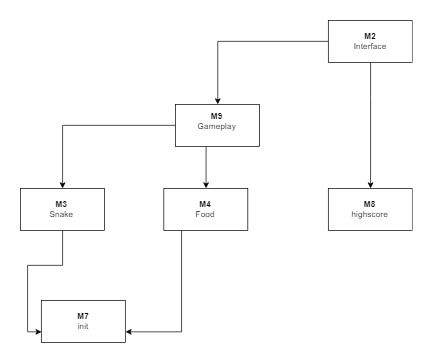
\includegraphics{Use_Heirarchy}
\label{FigUH}
\end{figure}

%\section*{References}

\bibliographystyle {plainnat}
\bibliography {MG}

\end{document}